\documentclass[a4paper]{article}

\usepackage[T1]{fontenc}
\usepackage[italian]{babel}
\usepackage[latin1]{inputenc}
\usepackage{graphicx}
\usepackage{float}
\usepackage[margin=2 cm]{geometry}
\usepackage{multirow}
\usepackage{multicol}
\usepackage{textcomp}
\usepackage{caption}
\usepackage{units}
\usepackage{amsmath}
\author{Alberto Bordin, Giulio Cappelli}
\title{Fibre ottiche}
\date{20-24 Novembre 2017}
\newcommand{\minitab}[2][l]{\begin{tabular}#1 #2\end{tabular}}


\begin{document}
	\maketitle
	
	\begin{abstract}
		 
	\end{abstract}
	
\section{Teoria}

\section{Apparato sperimentale}

\section{Apertura numerica}

\subsection{Teoria}

\subsection{Presa dati}

2 tabelle

\subsection{Analisi dati}

2 plot con interpolazione quadratica o al massimo cubica

\newpage
\section{Attenuazione}

\begin{multicols}{2}

\subsection{Teoria}
In una fibra ottica si ha dissipazione dovuta allo scattering Rayleigh con le impurit� della fibra. La potenza dissipata � proporzionale a $\lambda^{-4}$, scopo dell'esperienza � verificare questa legge di potenza.\\
L'attenuazione $\alpha$, che � proporzionale alla potenza dissipata, � definita come 
\[\alpha = \frac{10}{L} \log \left | \frac{ P_{in}}{P_{out}} \right | \quad\textrm{     [dB/km]}\]
dove $P_{in}$ e $P_{out}$ sono, rispettivamente, la potenza in ingresso e la potenza in uscita ad un tratto di fibra di lunghezza $L$.

\subsection{Apparato sperimentale}

\begin{figure}[H]
	\centering
	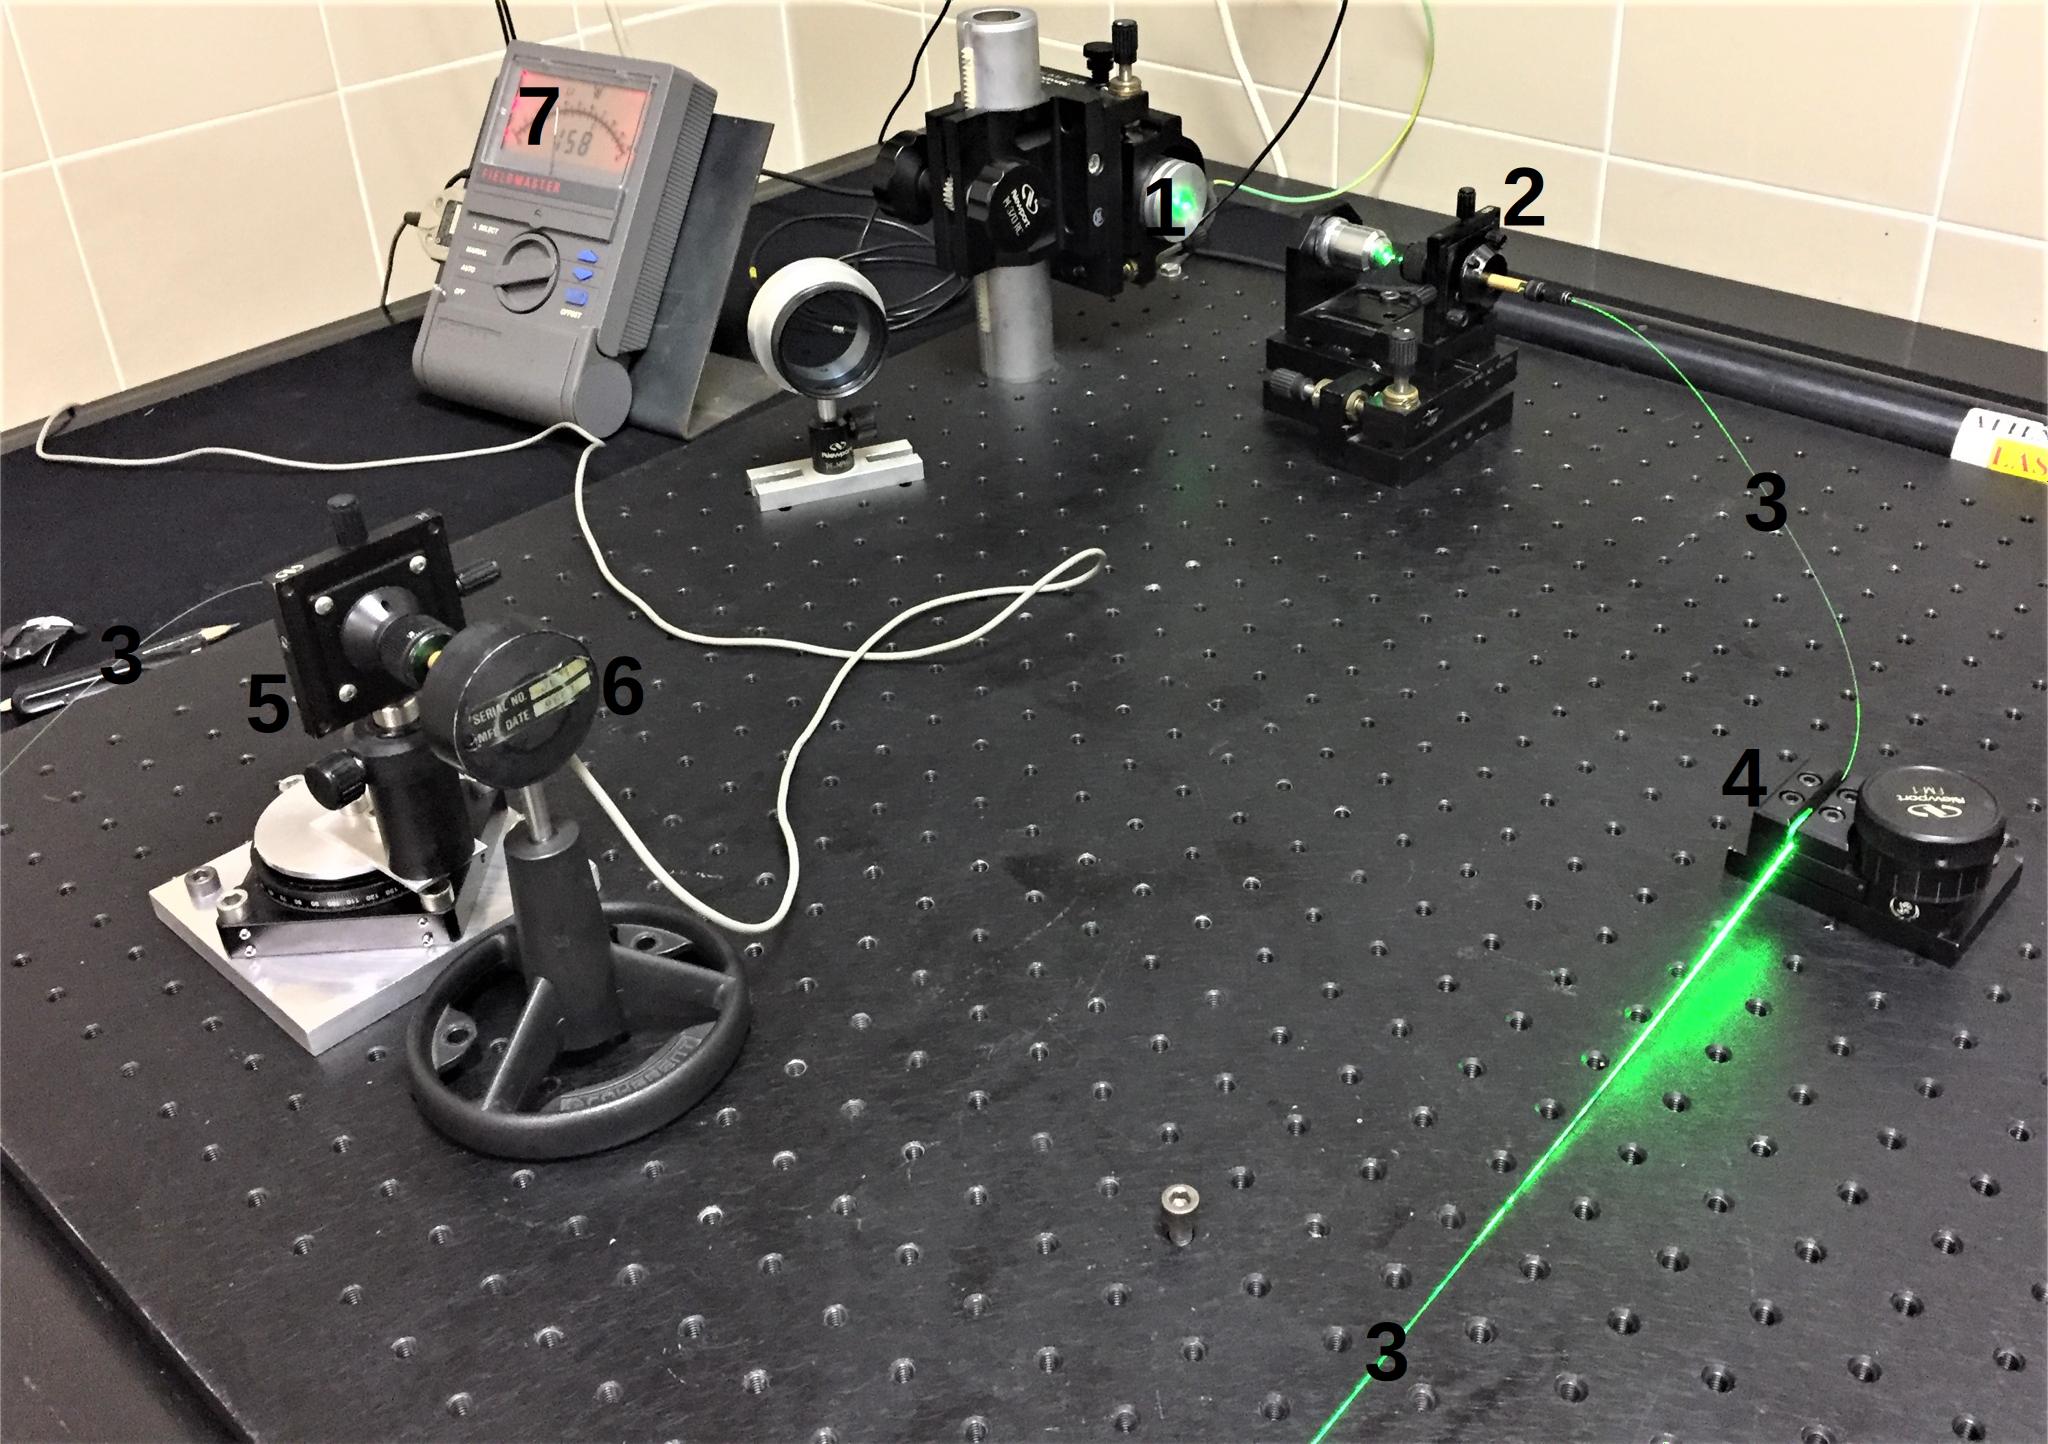
\includegraphics[width=0.5\textwidth]{apparato_attenuazione.pdf}
	\caption{Apparato sperimentale per la misura di attenuazione.}
	\begin{enumerate}
		\item Laser
		\item Lanciatore (con obiettivo 20x)
		\item Fibra ottica multimodo F-MLD
		\item \textit{Scrambler}: una sorta di piccola morsa ondulata che serve ad eliminare i modi spuri.
		\item Uscita della fibra
		\item Sensore del \textit{power meter}
		\item Schermo del \textit{power meter}
		\item Rotolo da $\sim300$ m di fibra ottica
	\end{enumerate}
	\label{fig:apparato_attenuazione}
	\begin{minipage}{0.23\textwidth}
		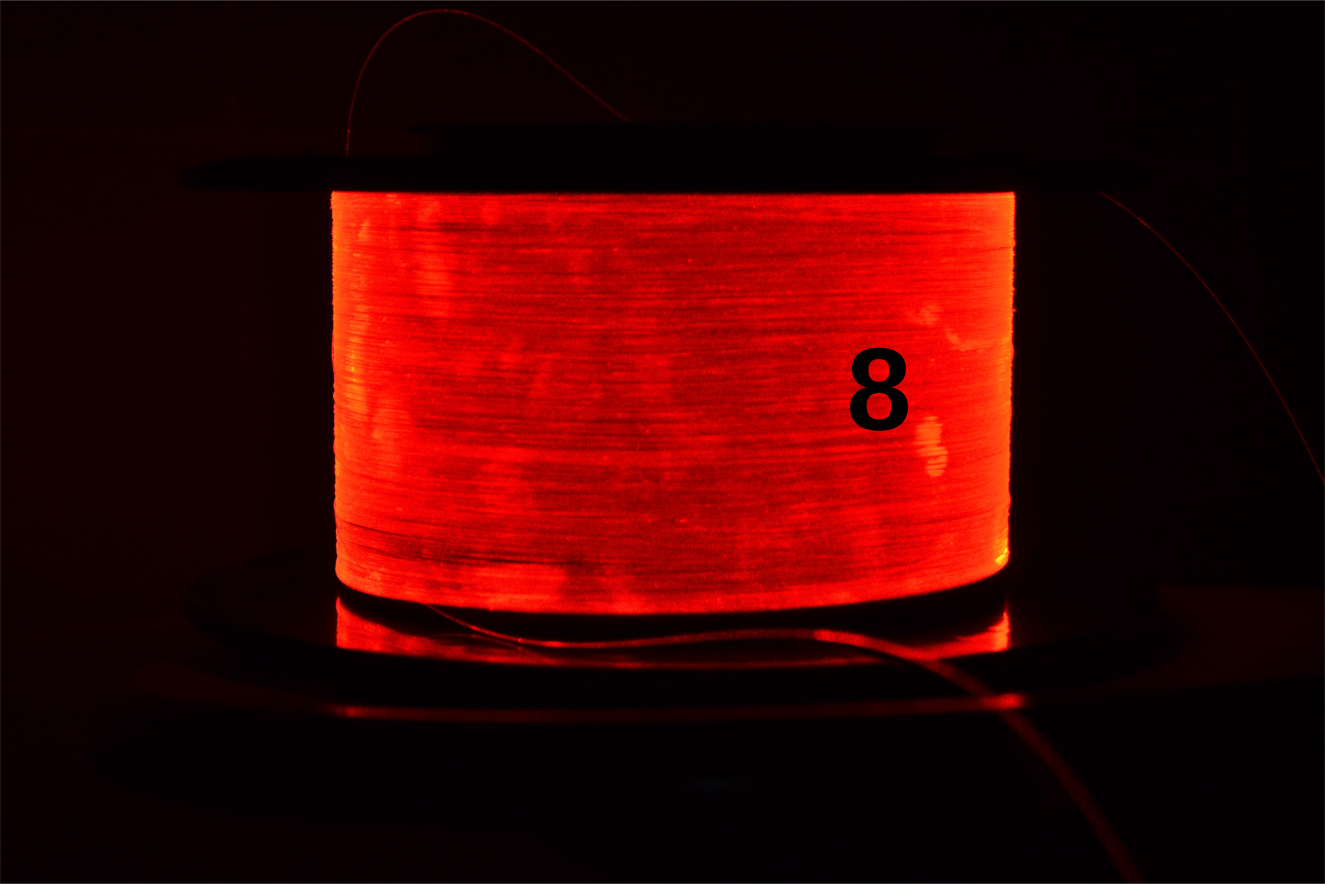
\includegraphics[width=\textwidth]{bobina_rossa.pdf}
	\end{minipage}
\begin{minipage}{0.24\textwidth}
	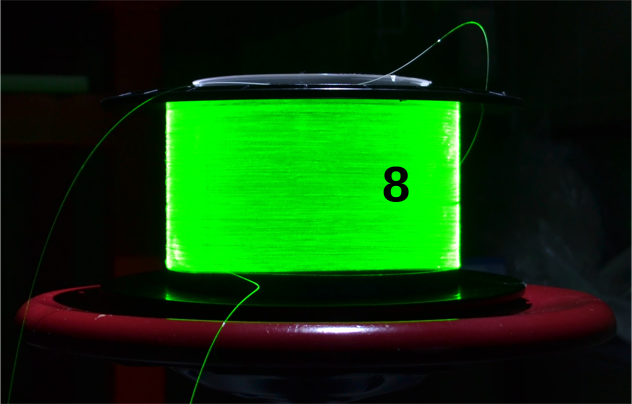
\includegraphics[width=\textwidth]{bobina_verde.pdf}
\end{minipage}
\end{figure}

\subsection{Presa dati}
La misura � svolta in due passaggi.
\begin{enumerate}
	\item Si lancia in fibra un fascio laser e si misura la potenza in uscita: $P_{out}$.
	\item Si taglia la fibra a 2 metri dal lanciatore e si misura di nuovo la potenza in uscita: $P_{in}$.
\end{enumerate}
Quindi $L$ � la lunghezza del rotolo meno i 2 m tagliati.

\begin{table}[H]
	\centering
	\begin{tabular}{|c|cccc|}
		\hline
		$\lambda$ [nm] & $L$ [m]  & $P_{out}$ [mW]& $P_{in}$ [mW]& $\alpha [dB/km]$ \\
		\hline
		633  & 293.5(5)? & 0.598(?) & 1.63(?) & \\
		
		532 & 291.3(5)? & 0.156(?) & 1.47(?) & \\
		\hline
		\hline
		633  & 289.2(5)? & 0.832(?) & 2.44(?) & \\
		
		532 & 287.1(5)? & 0.320(2) & 2.80(3) & \\
		\hline
		
		
	\end{tabular}
	\caption{.}
	\label{tab:alpha}
\end{table}
	
\subsection{Analisi dati}
	
4 plot: 1 normale e 1 loglog per 2 volte
	
\end{multicols}



\section{Propagazione modo LP$_{01}$ in una fibra SM}

\subsection{Teoria}

\subsection{Presa dati}

1 tabella

\subsection{Analisi dati}

1 plot

\section{Propagazione modi superiori}

\subsection{Teoria}

\subsection{Presa dati}

\subsection{Analisi dati}

\section{Fibra a conservazione di polarizzazione}

\subsection{Teoria}

\subsection{Presa dati}

\subsection{Analisi dati}

1 figura

\section{Lente GRIN}

\begin{multicols}{2}


\subsection{Teoria}
Una lente GRIN (da GRadient-INdex) � un cilindro fatto di materiale rifrangente con indice di rifrazione variabile a seconda della distanza dall'asse.
\begin{figure}[H]
	\centering
	\includegraphics[width=0.4\textwidth]{Grin-lens.png}
\end{figure}
Una lente GRIN tagliata a $\lambda/4$ focalizza assi parassiali sulla superficie e viceversa. La lente GRIN a nostra disposizione � tagliata a 0.29$\lambda$ quindi focalizza onde sferiche ad una certa distanza dalla superficie.

\subsection{Coefficiente di accoppiamento}
L'idea � usare la lente GRIN per lanciare luce in fibra. Misuriamo quindi il coefficiente di accoppiamento di una sorgente laser o LED a una fibra ottica multimodo attraverso una lente GRIN.
Il coefficiente di accoppiamento si ottiene con la formula
\[\Gamma = 10 \log\left |\frac{P_{in}}{P_{out}} \right|\]
\subsubsection*{Procedura e accorgimenti}
$P_{in}$ � la potenza in ingresso, misurata con il \textit{power meter} a diretto contatto con la sorgente, e $P_{out}$ � la potenza in uscita, misurata, con lo stesso \textit{power meter}, all'uscita della fibra ottica.

$P_{out}$ dipende dall'allineamento l'apparato, la sua misura non � quindi ripetibile a meno di non ottenere lo stesso identico allineamento. Pertanto abbiamo scelto, per convenzione, di variare l'allineamento fino a registrare il massimo valore di $P_{out}$, in questo modo altri studenti che utilizzino il nostro apparato e seguano la stessa procedura devono trovare il medesimo valore. Allo stesso modo $P_{in}$ � la massima potenza registrata con la sorgente a diretto contatto con il sensore.

La corrente di alimentazione varia lentamente in funzione del tempo (effetti $1/f$) quindi ci siamo assicurati che le misure di $P_{in}$ e $P_{out}$ avvenissero con la stessa alimentazione. La misura che richiede pi� pazienza � quella di $P_{out}$, quindi l'abbiamo misurata per prima e immediatamente dopo abbiamo misurato $P_{in}$, verificando che l'alimentatore fornisse la stessa corrente.

\subsubsection*{Risultati}
\begin{table}[H]
	\centering
	\begin{tabular}{|c|cccc|}
		\hline
		& $I_{in}$ [mA]  & $P_{out}$ [mW]& $P_{in}$ [mW]& $\Gamma [dB]$ \\
		\hline
		laser  & 78.0(1) & 3.50(1) & 6.19(6) & 2.48(4)\\

		LED & 81.1(2) & 0.00491(2) & 8.21(10) & 32.23(6)\\
		\hline
	\end{tabular}
	\caption{Coefficiente di accoppiamento. L'errore sulla corrente � la digitalizzazione, gli errori sulle potenze una nostra stima in base alle fluttuazioni delle misure.}
	\label{tab:GRIN}
\end{table}

In Tabella \ref{tab:GRIN} ci sono i dati raccolti ed il coefficiente di accoppiamento ricavato:
\begin{align*}
	\Gamma_{laser} &= 2.48(4) \textrm{ dB}\\
	\Gamma_{LED} &= 32.23(6) \textrm{ dB}
\end{align*}

\subsection{Trasmissione di un segnale}
Modulando l'intensit� della luce lanciata in fibra � possibile trasmettere un segnale.
\begin{figure}[H]
	\centering
	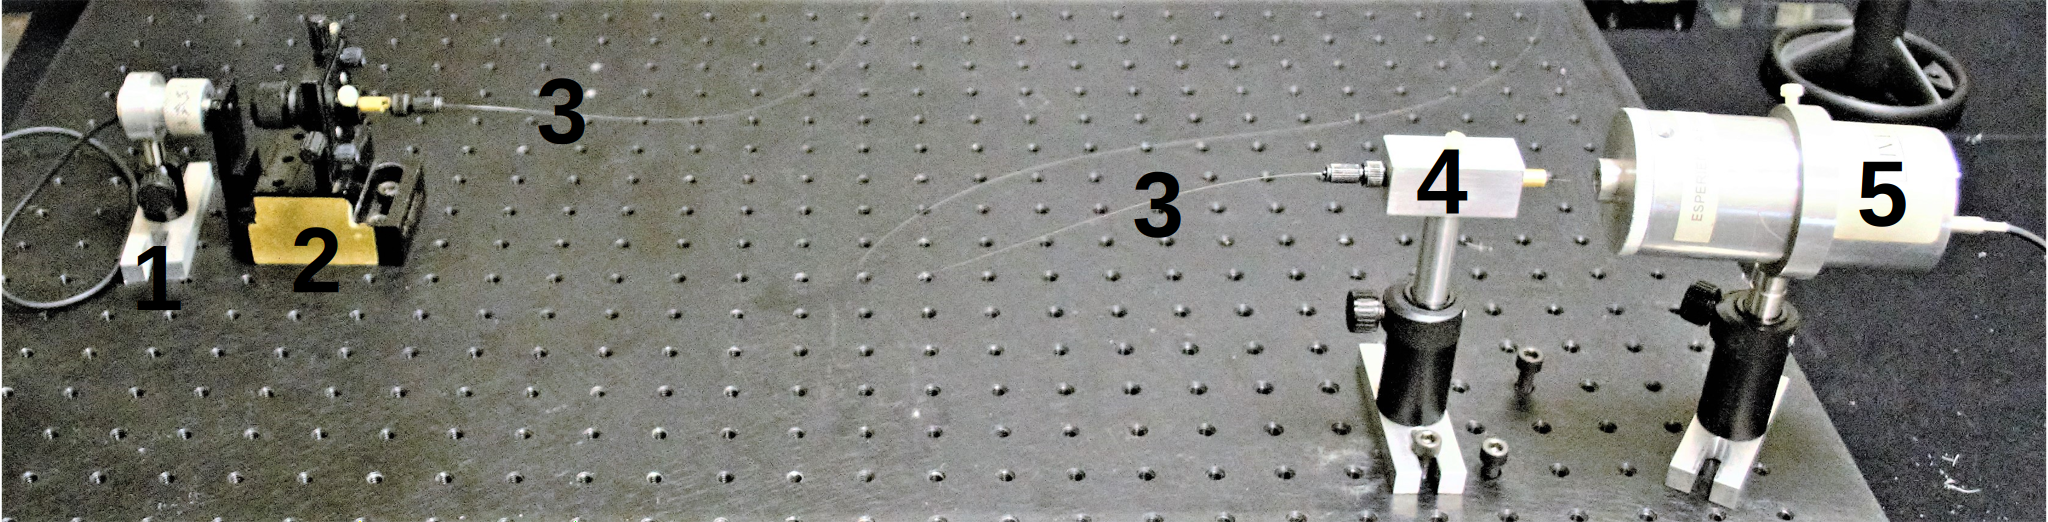
\includegraphics[width=0.5\textwidth]{apparato_segnale_acustico.pdf}
	\caption{Apparato sperimentale per la trasmissone di un segnale.}
	\begin{enumerate}
		\item Diodo laser
		\item Lanciatore (con lente GRIN)
		\item Fibra ottica
		\item Uscita della fibra
		\item Rilevatore al silicio
	\end{enumerate}
	\label{fig:apparato_segnale}
\end{figure}

In Figura \ref{fig:apparato_segnale} � rappresentato l'apparato sperimentale che utilizziamo. Il diodo laser � alimentato da una corrente modulata con un piccolo segnale prodotto da un generatore di funzioni.\\
Il rilevatore, che trasforma il segnale ottico in una tensione, � collegato ad un amplificatore che trasforma la tensione in segnale acustico, che sentiamo ad orecchio.

Registriamo il segnale acustico grazie ad un'app gratuita per cellulare per accordare gli strumenti musicali.
In Figura \ref{fig:segnale_acustico} sono riportati gli screenshot delle 3 misure effettuate:
\begin{enumerate}
	\item Segnale dato dalla luce ambientale. La stanza � illuminata da lampade al neon, che viene eccitato al doppio della frequenza della corrente alternata, quindi circa a 100-120 Hz. Misuriamo 98 Hz.
	\item Segnale del generatore di funzioni: regoliamo la frequenza fino ad intonare un la5 (880 Hz).
	\item Segnale del generatore di funzioni: regoliamo la frequenza fino ad intonare un la4 (440 Hz).
\end{enumerate}

\begin{figure}[H]
	\centering
	\begin{minipage}{0.148\textwidth}
		\includegraphics[width=\textwidth]{sol2.png}
	\end{minipage}
	\begin{minipage}{0.16\textwidth}
		\includegraphics[width=\textwidth]{la5.png}
	\end{minipage}
	\begin{minipage}{0.16\textwidth}
		\includegraphics[width=\textwidth]{la4.png}
	\end{minipage}
	\caption{Screenshot del cellulare che misura la frequenza, cerchiata in rosso.}
	\label{fig:segnale_acustico}
\end{figure}

\end{multicols}
	
\end{document}